\section{Methodology}

\subsection{Datasets}
One of the major challenges in Sentiment Analysis of Twitter is to collect a labeled dataset.
Researchers have made public the following datasets for training and testing classifiers.

\subsubsection{Twitter Sentiment Corpus}
This is a collection of 5513 tweets collected for four different topics, namely, Apple, Google, Microsoft, Twitter
It is collected and hand-classified by Sanders Analytics LLC \cite{SA}.
Each entry in the corpus contains, Tweet id, Topic and a Sentiment label.
We use Twitter-Python library to enrich this data by downloading data like Tweet text, Creation Date, Creator etc. for every Tweet id. %%ref Twitter-Python Library
Each Tweet is classified by an American male into the following four categories.

\begin{description}
	\item[Positive] {For showing positive sentiment towards the topic}
	\item[Positive] {For showing no or mixed or weak sentiments towards the topic}
	\item[Negative] {For showing negative sentiment towards the topic}	
	\item[Irrelevant] {For non English text or off-topic comments}
	{For showing positive sentiment towards the topic}
\end{description}

\begin{table}[h]
\centering
	\begin{tabular}{| p{0.75\textwidth} | l | }
	\hline
		\multicolumn{1}{|c|}{Tweet} &
		\multicolumn{1}{|c|}{Classification} \\
	\hline
	\verb'S/O to @apple for replacing my phone for free...' &  \verb'positive' \\ \hline
	
	\verb"+1  RT @Doug_Newton: @apple PLEASE FIX #Siri!!!!" {...}
	\verb"She can't connect to your network!!!!!!!" &  \verb'negative' \\ \hline
	
	\verb'Apple Users Get The official Kalifornia Cavi App' {...}
	\verb'on your Apple Device now on  - powered by @Apple' {...}
	\verb'- Download it free http://t.co/HlGnvlRw' &  \verb'neutral' \\ \hline
	
	\end{tabular}
\caption{Classification of Tweets by sentiments expressed in each}
\label{table:twt}
\end{table}

\subsubsection{Stanford Twitter}
This is a collection of 100000 tweets labeled 0 (negative), 2 (neutral) or 4 (positive).
This data was automatically annotated, not by human.
The authors assume that any tweet with positive emoticon like \verb':)' were positive
	and the tweets with negative emoticon like \verb':(' were negative \cite{S140}.

\subsection{Features}
A wide variety of features can be used to build a classifier for tweets.
The most widely used and basic feature set is word n-grams.
However, there's a lot of domain specific information present in tweets that can also be used for classifying them.
Preprocessing is needed to normalise these features. Relevant preprocessing methods are discussed below.

\subsubsection{Pre Processing}

User-generated content on the web is seldom present in a form usable for learning.
It becomes important to normalise the text by applying a series of preprocessing steps.
In this paper we have applied an extensive set of preprocessing steps to
	decrease the size of the feature set to make it suitable for learning algorithms.

\begin{table}[h]
\centering
	\begin{tabular}{|l|l|l|}
	\hline
	Step & Number & Percent	\\
	\hline
	before preprocessing & 19128 & \\
	\hline
	after processing Hashtags & 18649 & 97.50\% \\
	after processing Handles & 17118 & 89.49\% \\
	after processing Urls & 16723 & 87.43\% \\
	after processing Emoticons & 18631 & 97.40\% \\
	after processing Punctuations & 13724 & 71.75\% \\
	after processing Repeatings & 18544 & 96.95\% \\
	\hline
	after processing All & 11031 & 57.67\% \\
	\hline
	\end{tabular}
\caption{Number of words before and after pre-processing}
\label{table:preproc_numwords}
\end{table}

We have started by removing the query terms from the text.
This is important so that no particular query word becomes a feature in our classifier.
Next we have removed links, including URLs, Handles and Hashtags.
A particular URL is not important. However, presence of a URL can be an important feature for classification.
We give below a description of some popular features present in tweet text.

	\begin{description}
	\item[Hashtags]{A hashtag is a word or an un-spaced phrase prefixed with the hash symbol (\#)
					These are used to both naming subjects and phrases that are currently in trending topics.
					For example, \verb+#iPad+, \verb+#news+}
	\item[Handles]{Every Twitter user has a unique username.
					Any thing directed towards that user can be indicated be writing their username preceded by \@.
					Thus, these are like proper nouns.
						For example, \verb+@Apple+}
	\item[Emoticons]{Keyboard written pictorial representation of a facial expression,
						used to draw a receiver's attention to the temper of sender's nominal verbal communication,
						thus changing and improving its interpretation.
					Table \ref{table:emot} lists the emoticons currently identified.} %% REF: http://en.wikipedia.org/wiki/Emoticon
	\end{description}

These features are identified using regular expressions and replaced by a single word.
Table \ref{table:preproc_numwords} lists the decrease in feature set due to processing each of these features.
Table \ref{table:preproc_freq} illustrates the frequency of these features per tweet.
A brief description of the preprocessing steps is given below.

\begin{table}[h]
\centering
	\begin{tabular}{|l|l|l|}
	\hline
	Feature    & Avg & Max \\
	\hline
	Handles    & 0.6761 & 8 \\
	Hashtags   & 2.028 & 13 \\
	Urls       & 0.4431 & 4 \\
	Emoticons  & 0.05500 & 3 \\
	\hline
	\end{tabular}
\caption{Frequency of Features per Tweet}
\label{table:preproc_freq}
\end{table}

\begin{table}[h]
\centering
	\begin{tabular}{|l|llllll|}
	
	\hline
		\multicolumn{1}{|c|}{Emoticons} &
		\multicolumn{6}{|c|}{Examples} \\
	\hline
	\verb+EMOT_SMILEY+ 	& \verb+:-)+ 	& \verb+:)+ 	& \verb+(:+ 	& \verb+(-:+ 	& \verb++ 	& \verb++ \\
	\verb+EMOT_LAUGH+ 	& \verb+:-D+ 	& \verb+:D+ 	& \verb+X-D+ 	& \verb+XD+ 	& \verb+xD+ 	& \verb++ \\
	\verb+EMOT_LOVE+ 	& \verb+<3+ 	& \verb+:*+ 	& \verb++ 	& \verb++ 	& \verb++ 	& \verb++ \\
	\verb+EMOT_WINK+ 	& \verb+;-)+ 	& \verb+;)+ 	& \verb+;-D+ 	& \verb+;D+ 	& \verb+(;+ 	& \verb+(-;+ \\
	\verb+EMOT_FROWN+ 	& \verb+:-(+ 	& \verb+:(+ 	& \verb+(:+ 	& \verb+(-:+ 	& \verb++ 	& \verb++ \\
	\verb+EMOT_CRY+ 	& \verb+:,(+ 	& \verb+:'(+ 	& \verb+:"(+ 	& \verb+:((+ 	& \verb++ 	& \verb++ \\
	\hline
	
	\end{tabular}
\caption{List of Emoticons}
\label{table:emot}
\end{table}

Although not all Punctuations are important from the point of view of classification but some of these,
	like question mark, exclamation mark can also provide information about the sentiments of the text.
We replace every word boundary by a list of relevant punctuations present at that pont.
Table \ref{table:punc} lists the punctuations currently identified
As a final step, we replace charachters repeating more than twice as two charachters.
This takes care of words like hurrryyyyy, yaaayyyyy often present in user-generated content on the internet.

\begin{table}[h]
\centering
	\begin{tabular}{|l|ll|}
	
	\hline
		\multicolumn{1}{|c|}{Punctuations} &
		\multicolumn{2}{|c|}{Examples} \\
	\hline
	\verb+PUNC_DOT+ & \verb+.+ & \verb++ \\
	\verb+PUNC_EXCL+ & \verb+!+ & \verb+¡+ \\
	\verb+PUNC_QUES+ & \verb+?+ & \verb+¿+ \\
	\verb+PUNC_ELLP+ & \verb+...+ & \verb+…+ \\
	\hline

	\end{tabular}
\caption{List of Punctuations}
\label{table:punc}
\end{table}

\subsubsection{n-grams}

Word unigrams are the simplest features are being used for sentiment analysis of tweets data.
Models trained from word unigrams were shown to outperform random classifiers by a decent margin of 20\% \cite[SHA].
To build our first baseline model, we have used Naive Bayes' Classifier trained on word unigrams.
Figure \ref{fig:unigrams} illustrates the most frequent word unigrams in our dataset.

\subsubsection{Other Features}

Research papers in this field describe other features that can be used.
Among these, the most important are Part-of-Speech tagging (POS).
For each tweet, number of verbs, adverbs, adjectives, nouns, and any other parts of speech can be counted and made into a feature\cite{KWM}.
Emoticons, Abbreviations, and intensifiers (e.g., all-caps and character repetitions) can also be used to further improve the results \cite{KWM}.

\begin{figure}[h]
\centering
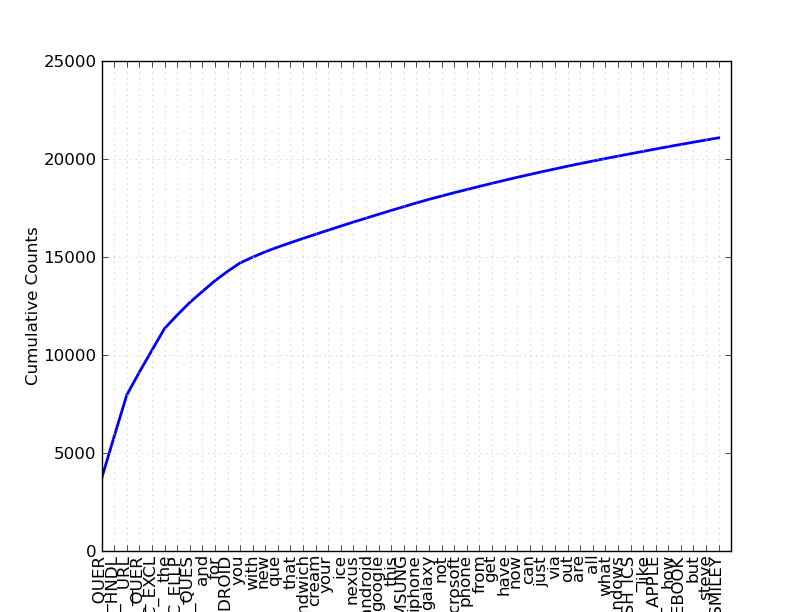
\includegraphics[width=\textwidth]{img/fdist-unigrams.png}
\caption{Cumulative Frequency Plot for 50 Most Frequent Words}
\label{fig:unigrams}
\end{figure}

Based on previous research \cite{survey}, it is not clear whether higher-order n-grams are useful features or not.
For example, some researchers report that unigrams outperform bigrams when classifying movie reviews by sentiment polarity,
while others find that in some settings, bigrams and trigrams yield better product-review polarity classification.
We proceed to test the most frequent bigrams and trigrams.

\begin{figure}[h]
\centering
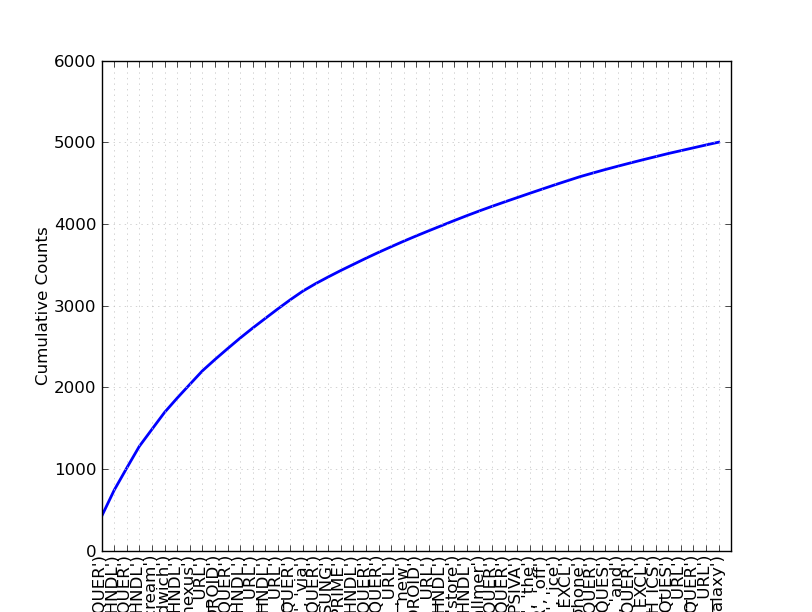
\includegraphics[width=\textwidth]{img/fdist-bigrams.png}
\caption{Cumulative Frequency Plot for 50 Most Frequent Word Bigrams}
\label{fig:bigrams}
\end{figure}

\begin{figure}[h]
\centering
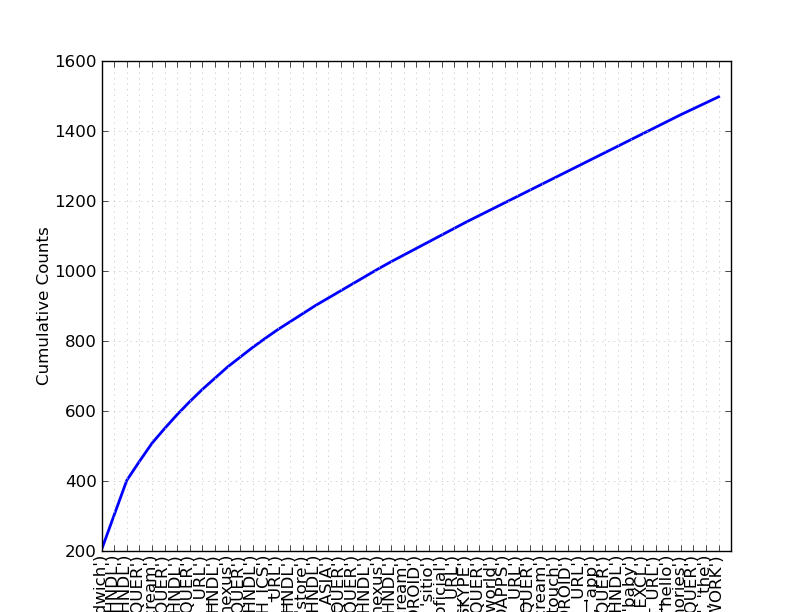
\includegraphics[width=\textwidth]{img/fdist-trigrams.png}
\caption{Cumulative Frequency Plot for 50 Most Frequent Word Trigrams}
\label{fig:trigrams}
\end{figure}

From the list of most frequent word bigrams and trigrams, it is not completely apparent if these features will be helpful
	for classification or not.
We can consider some of most frequent of these for features and test our classifier with those.
And then we can compare the results vis-a-vis unigrams.

\subsection{Experimentation}
We train a multi-class classifier that categorises a tweet into positive, neutral or negative.
We break our data into training and testing sets with a ratio of \verb'9:1'.
The classifier was trained using Naive Bayes model. %, Maximum Entropy and Decision Tree Model.
Previous works have shown that applying machine learning techniques based on unigram models can achieve over \verb'80%' in accuracy \cite{survey}
We were able to get a an accuracy of \verb'83.92%'.
Thus we can say that our classifier performs at par with the state of the around result.
Figure \ref{fig:naive_accuracy} illustrates the confusion matrix and accuracy of our classifier.
In Table \ref{table:naive_features}, top classifying features are listed.
It can be noticed from the features that we have good results.

\begin{figure}[h]
\centering
\begin{varwidth}[t]{\textwidth}
	\begin{verbatim}
Accuracy : 0.839248434238

Confusion Matrix
    |   n   n   p |
    |   e   e   o |
    |   g   u   s |
----+-------------+
neg |  <8> 39   . |
neu |   2<393>  . |
pos |   .  36  <1>|
----+-------------+
	\end{verbatim}
\end{varwidth}
\caption{Naive Bayes Statistics}
\label{fig:naive_accuracy}
\end{figure}

\begin{table}[h]
\centering
\begin{tabular}{|l|l|l|}
\hline
Feature & Classification & Odds \\
\hline
\verb'        contains(fix) = True' & \verb'neg : neu' & \verb'76.8 : 1.0' \\
\verb'       contains(hate) = True' & \verb'neg : neu' & \verb'67.5 : 1.0' \\
\verb'   contains(eclipsed) = True' & \verb'neg : neu' & \verb'48.9 : 1.0' \\
\verb'    contains(restore) = True' & \verb'neg : neu' & \verb'48.9 : 1.0' \\
\verb'     contains(loving) = True' & \verb'pos : neu' & \verb'47.8 : 1.0' \\
\verb'        contains(wtf) = True' & \verb'neg : neu' & \verb'39.6 : 1.0' \\
\verb'    contains(amazing) = True' & \verb'pos : neu' & \verb'35.6 : 1.0' \\
\verb'     contains(issues) = True' & \verb'neg : neu' & \verb'34.9 : 1.0' \\
\verb'       contains(blue) = True' & \verb'neg : neu' & \verb'34.9 : 1.0' \\
\verb'      contains(sucks) = True' & \verb'neg : neu' & \verb'34.9 : 1.0' \\
\verb' contains(impressive) = True' & \verb'pos : neu' & \verb'27.7 : 1.0' \\
\verb'     contains(charge) = True' & \verb'neg : neu' & \verb'25.6 : 1.0' \\
\verb'       contains(dead) = True' & \verb'neg : neu' & \verb'25.6 : 1.0' \\
\verb'    contains(missing) = True' & \verb'neg : neu' & \verb'25.6 : 1.0' \\
\verb'contains(reservation) = True' & \verb'neg : neu' & \verb'25.6 : 1.0' \\
\verb'      contains(since) = True' & \verb'neg : neu' & \verb'24.9 : 1.0' \\
\verb'        contains(won) = True' & \verb'neg : neu' & \verb'23.7 : 1.0' \\
\verb'      contains(fixed) = True' & \verb'neg : neu' & \verb'23.7 : 1.0' \\
\verb'   contains(replaced) = True' & \verb'pos : neu' & \verb'22.6 : 1.0' \\
\verb'      contains(usage) = True' & \verb'pos : neu' & \verb'22.6 : 1.0' \\
\hline
\end{tabular}
\caption{Best Classification Features for Naive Bayes Classifier}
\label{table:naive_features}
\end{table}

%\begin{table}[h]
%\centering
%Maximum Entropy Statistics here
%\caption{Maximum Entropy Statistics}
%\label{maxent}
%\end{table}

%\begin{table}[h]
%\centering
%Decision Tree Statistics here
%\caption{Decision Tree Statistics}
%\label{dtree}
%\end{table}


